\section{Punti di estensione} \label{section:punti_estensione}

ShopChain è un'applicazione progettata pensando anche ad eventuali operazioni future di manutenzione o
estensione del prodotto: durante lo sviluppo dell'applicazione ShopChain sono stati esplorati vari spunti per nuove features e ampliamenti, 
che però a causa del poco tempo rimasto non sono state implementate in tempo.
Sono state individuate principalmente tre macro aree che potranno essere ampliate.

\subsection{Smart Contract}

\subsubsection{Conversione a stable coin}

La funzionalità di convertire l'ammontare depositato sul contratto in stable coin è un'interessante funzionalità che il gruppo ha individuato. Per limiti 
di tempo e costi legati al progetto, non è stata implementata in tutti i suoi punti, ma è stata affrontata sul lato smart contract.\\
Il gruppo ha condotto quindi uno studio relativamente ai passaggi da affrontare per attuare il meccanismo di conversione dei token\glo{}.
Prima di procedere è necessario descrivere e comprendere alcune componenti fondamentali che saranno necessarie:

\begin{itemize}
    \item Wrapped FTM: è un token crypto ancorato al valore del Fantom. Viene chiamato così oerchè l'asset originale viene messo in un wrapper che consente di crearne una versione su un'altra blockchain. Questo permette di creare ponti tra diverse blockchain e utilizzare asset non nativi su  un'altra blockchain. Ovviamente in genere può essere riscattato per il corrispettivo in qualsiasi momento. Il processo di "wrapping" permette quindi di rendere il token Fantom conforme allo standard ERC-20 e poter essere, ad esempio nel nostro caso, convertito;
    \item Stable Coin: è un token che ha valore fissato con un rapporto 1:1 con una valuta FIAT\glo{};
    \item Liquidity Pool: è un insieme di fondi bloccati in uno smart contract che generalmente contengono due token diversi. Hanno diversi casi d'uso tra cui la possibilità di fungere da punto di scambio tra i due token;
    \item Factory Contract: è un contratto che si occupa di gestire ed eseguire oprazioni sulle coppie di token. In particolare la sua funzione principale è quella di creare uno smart contract associato alla coppia di token scelta. Quest'ultima funzione è necessaria se si vuole generare una propria liquidity pool;
    \item Router Contract: è un contratto che fornisce un supporto a tutte quelle che sono le funzionalità di trading dei token e gestione della liquidità.
\end{itemize}

Le componenti citate sono fondamentali per poter effettuare la conversione in stable coin. 
Il gruppo ha deciso di sviluppare un primo PoC di questa funzionalità direttamente sulla rete fantom di test. La rete di test presenta però delle mancanze rispetto alla rete principale, vengono a mancare infatti i contratti di alcuni token, come ad esempio USDT (scelto dal gruppo), e quelli che si occupa di gestire le liquidity pool di WFTM e eventuali stable coin.
Il gruppo ha deciso di creare un token che simuli il comportamento di USDT (è possibile visualizzare il contratto associato al seguente link):

\href{}{link}

Purtroppo non è possibile replicare il funzionamento di un vero USDT e il suo relativo vincolo al valore del dollaro, ma è sufficiente per dimostrare come avvenga il processo di conversione.\\

Sulla rete Fantom il provider dei contratti per la gestione delle coppie di token e delle pool di liquidità è SpookySwap. In particolare come anticipato, è necessario riferirsi ai due contratti UniswapV2Factory (Contract Factory) e UniswapV2Router02 (Contract Router), è possibile visualizzarne i riferimenti al seguente link della documentazione:

\begin{center}
    \href{https://docs.spooky.fi/Resources/contracts}{https://docs.spooky.fi/Resources/contracts}
\end{center}

Tramite il contratto UniswapV2Factory abbiamo creato la pair WFTM/USDT (usando il token ERC-20 da noi creato).\\ Dopo aver creato la coppia è stata generata la corrispondente liquidity pool in cui è possibile fornire o rimuovere liquidità. 
è importante ricordare che il valore del token USDT da noi creato è associato al rapporto delle quantità dei due token presenti nella pool e non al dollaro.\\

A questo punto abbiamo proceduto ad inserire all'interno del contratto la chiamata al contratto UniswapV2Router02 per effettuare la conversione tra i due token.
Il metodo da chiamare è UniswapV2Router02.swapETHForExactTokens, che prende in input:

\begin{itemize}
    \item Equivalente di USDT da richiedere alla pool;
    \item Array contente gli indirizzi dei due contratti dei due token;
    \item Indirizzo a cui ritornare gli USDT richiesti (in questo caso è necessario indicare l'indirizzo del contratto);
    \item Un timestamp che indichi il timeout dopo il quale la transazione deve essere annullata.
\end{itemize}

Per approfondire ulteriormente il metodo, si veda la relativa documentazione:

\begin{center}
    \href{https://docs.uniswap.org/protocol/V2/reference/smart-contracts/router-02\#swaptokensforexacttokens}{https://docs.uniswap.org/protocol/V2/reference/smart-contracts/router-02\#swaptokensforexacttokens}
\end{center}

Poichè la conversione viene effettuata dal router su una pool, che verrà utilizzata da più utenti, il valore della conversione può cambiare rapidamente anche solo di poco. Il router in tal caso tornerà un ammontare di FTM da restituire al mittente della transazione nel caso in cui la conversione sia a suo sfavore. è necessario tenere traccia di questo comportamento e gestire la restituzione di tale importo.

%{screen con il codice}


\subsubsection{TheGraph protocol}

Nella pagina di visualizzazione degli ordini il gruppo ha implementato la possibilità di filtrare gli ordini restituiti direttamente dalla blockchain. Attualmente questa funzionalità è fornita solo tramite un controllo a front-end, in futuro si potrebbe evolvere la funzione di filtraggio tramite l'implementazione del protocollo TheGraph\glo.

The Graph è un protocollo decentralizzato per indicizzare e successivamente effettuare query dei dati presenti in blockchain in una modalità simile a quella che avviene con una normale base di dati. Questo permette di interrogare la blockchain in modo facile e veloce, ed estraendo dati che altrimenti non sarebbe possibile visualizzare.

In particolare quanto citato è possibile tramite la creazione di subgraph. Un sottografo non è altro che una serie di parametri necessari al protocollo per poter mappare e creare un indice dei dati presenti in blockchain.\\
Si compongono di tre componenti principali:

\begin{itemize}
 \item Manifest (subgraph.yaml) che definisce quali dati il sottografo andrà a indicizzare;

 \begin{figure}[H]
    \centering
    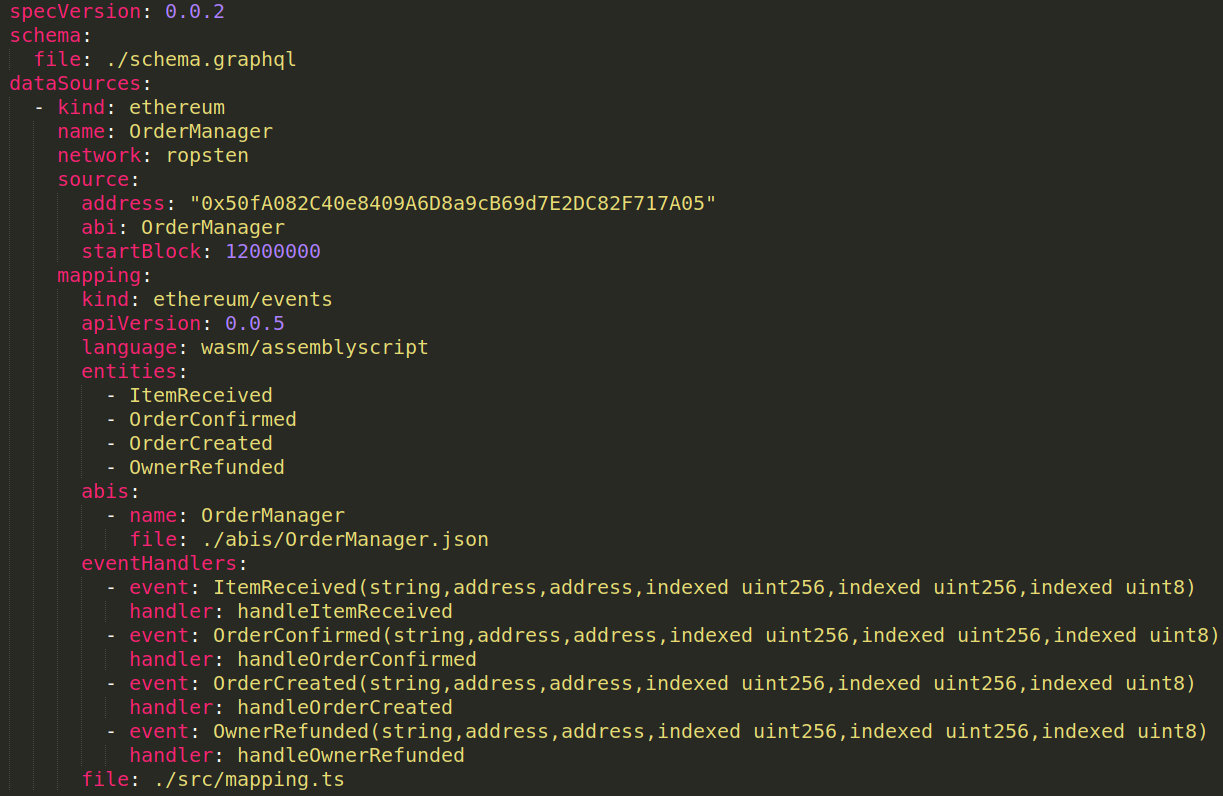
\includegraphics[scale=0.3]{immagini/subgraf.png}
    \caption{Esempio di un possibile subgraph configurato per il contratto OrderManager per la rete Ropsten.}
 \end{figure}


 \item Schema (schema.graphql) che riporta quali dati si desiderà ricevere dal sottografo;

 \begin{figure}[H]
    \centering
    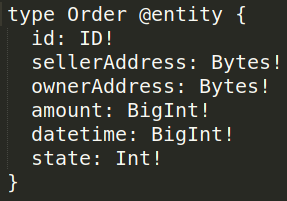
\includegraphics[scale=0.4]{immagini/schema.png}
    \caption{Esempio di file schema per la definizione entità Order.}
 \end{figure}

 \item AssemblyScript Mappings (mapping.ts) file che riporta la traduzione dei dati presenti in blockchain che il sottografo dovrà indicizzare.

 \begin{figure}[H]
    \centering
    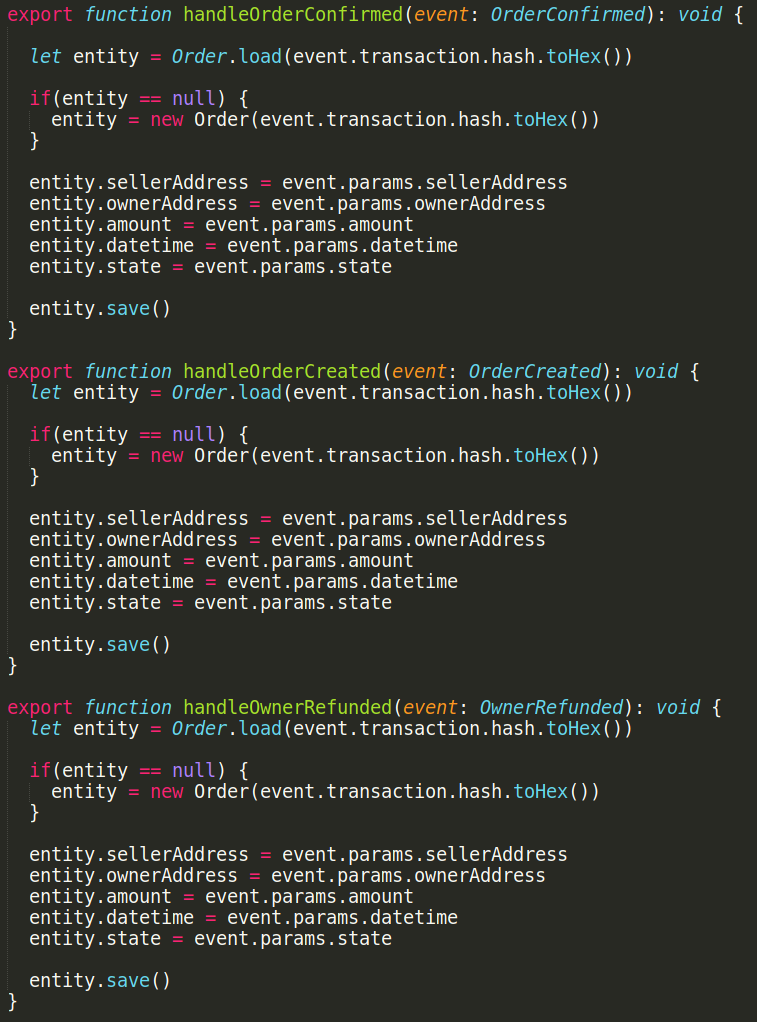
\includegraphics[scale=0.3]{immagini/map.png}
    \caption{Esempio di file mapping per l'indicizzazione degli eventi.}
 \end{figure}

\end{itemize}

Questa funzionalità non è stata portata avanti perchè non è disponibile sulla testnet di Fantom, ma solo sulla mainnet. Se la si vuole implementare sarà quindi necessario eseguire lo sviluppo e i relativi test su una testnet di Ethereum in cui è disponibile il protocollo (es. Rinkeby\glo). Una volta che lo sviluppo sarà finito si potrà procedere a caricare il subgraph creato sulla mainnet di Fantom senza particolari modifiche, poichè quest'ultima è una blockchain EVM.


\subsection{Chain differenti}

Un ovvio ampliamento per l'applicazione è il supporto a più blockchain, per raggiungere un bacino di utenza più ampio e garantire quindi un maggior successo dell'applicazione.\\


\subsection{Frontend}

\subsubsection{Immagine MoneyBox}

Il gruppo aveva pensato di associare ad ogni MoneyBox una immagine generata automaticamente, o presa da un pool di immagini definito. Se si sceglie di generarla automaticamente, si può prendere come seed di generazione uno tra i seguenti: l'id dell'ordine associato alla MoneyBox, 
il numero del blocco relativo alla transazione in blockchain, il timestamp della creazione.
Questo contribuisce ad una maggiore sicurezza nel condividere il link alla suddetta MoneyBox con amici, che potranno vedere a colpo d'occhio se il link è corretto tramite l'immagine incorporata.

\subsubsection{Riflettere i cambiamenti del contratto}

Con i cambiamenti che possono venire apportati agli smartcontract è bene che il lato frontend dell'applicazione sia aggiornato di conseguenza.
Nel caso dei cambiamenti proposti finora i cambiamenti individuati sono i seguenti:
\begin{itemize}
    \item \textbf{Stable Coin}: nelle pagine di pagamento, di dettaglio dell'ordine e di dettagli della MoneyBox, viene mostrato anche l'ammontare in stable coin dei vari pagamenti, per una migliore visione dei costi da parte dell'utente;
    \item \textbf{TheGraph}: le due pagine di elenco transazioni dovranno essere modificate per sfruttare appieno tutte le funzionalità portate dalla implementazione dei protocolli TheGraph;
    \item \textbf{Chain differenti}:  in un pop-up all'ingresso dell'applicazione, l'utente potrà selezionare la chain (e quindi la cryptovaluta correlata) con la quale procedere al pagamento. Tale scelta dovrà essere riportata anche nella breadcrumb come reminder testuale.
\end{itemize}

